\section{Безопасность в статистических БД}

\subsection{Определение статистической базы данных}

Статистическая база данных — это специализированный тип базы данных, который разработан и оптимизирован для хранения и управления статистическими данными. Она представляет собой совокупность таблиц, где каждая таблица содержит переменные (столбцы), представляющие различные характеристики или атрибуты, и наблюдения (строки), представляющие отдельные единицы данных или объекты. Статистические базы данных часто содержат большие объемы данных, собранных из различных источников, таких как опросы, эксперименты, наблюдения и административные записи. Такие базы данных могут содержать разнообразные типы данных, включая числовые, категориальные, временные ряды и многие другие. Они могут быть созданы и использованы для различных целей, таких как проведение исследований, анализ данных, подготовка отчетов, прогнозирование и принятие решений.
\\

Примеры статистических баз данных включают базы данных, содержащие данные о населении, экономические данные, данные о заболеваемости, результаты опросов и т.д. Эти базы данных могут быть созданы и поддерживаться различными организациями, такими как статистические агентства, исследовательские институты, университеты и государственные учреждения.
\\

Статистические базы данных обычно имеют стандартизированную структуру и формат, чтобы обеспечить согласованность и удобство использования данных для статистического анализа. Они также могут включать механизмы для обновления данных, контроля качества данных и обеспечения конфиденциальности и безопасности информации.
\\

Основные характеристики статистических баз данных включают:
\begin{enumerate}
    \item \textbf{Структуру данных:} статистические базы данных имеют четко определенную структуру, которая организует данные в таблицы, где каждая таблица представляет конкретную сущность данных или переменную. Структура включает поля (столбцы), представляющие различные атрибуты или характеристики, и записи (строки), представляющие отдельные экземпляры данных.
    \item \textbf{Интеграцию данных:} статистические базы данных могут интегрировать данные из нескольких источников для создания комплексного набора данных для анализа. Этот процесс интеграции включает сопоставление и преобразование данных для обеспечения согласованности и совместимости.
    \item \textbf{Качество данных:} обеспечение качества данных имеет важное значение в статистических базах данных. Они используют механизмы проверки данных, их очистки и стандартизации для минимизации ошибок, несогласованностей и пропущенных значений, которые могут повлиять на достоверность статистического анализа.
    \item \textbf{Метаданные:} статистические базы данных часто включают метаданные, которые содержат информацию о данных, такую как определения переменных, источники данных, методы сбора данных и любые преобразования, примененные к данным.
    \item \textbf{Политики безопасности и конфиденциальности:} статистические базы данных работают с конфиденциальными данными, такими как информация о персональных данных, банковские данные, бухгалтерские ведомости и подобными, и поэтому должны иметь меры безопасности для защиты конфиденциальности. Часто используются контроль доступа и методы анонимизации для обеспечения конфиденциальности данных.
\end{enumerate}


Статистические базы данных служат ценным ресурсом для исследователей, аналитиков и принимающих решения. Они позволяют выполнять различные статистические операции, такие как агрегирование, корреляция, регрессия и проверка гипотез, для выявления паттернов, взаимосвязей и тенденций в данных.
\\

Статистические базы данных позволяют проводить анализ данных, отвечать на исследовательские вопросы и принимать информированные решения на основе фактов. Они являются основой для множества статистических исследований, позволяя исследователям изучать различные явления, разрабатывать статистические модели и предсказывать будущие события.
\\

Примеры статистических баз данных могут включать базы данных национальных статистических агентств, таких как Федеральное агентство по статистике (Росстат) или Бюро экономического анализа (BEA) в США. Эти базы данных содержат широкий спектр статистической информации о населении, экономике, здравоохранении, социальных показателях и других аспектах жизни.
\\

Важно отметить, что статистические базы данных могут иметь различные спецификации и структуры, в зависимости от конкретной области знаний и целей использования данных.


\subsection{Классификация статистических баз данных}

Статистические базы данных можно классифицировать по различным критериям. Вот несколько основных классификаций статистических баз данных:
\\

\begin{enumerate}
    \item \textbf{По источнику данных:} \begin{itemize}
        \item Государственные статистические базы данных: это базы данных, содержащие статистическую информацию, собранную и поддерживаемую государственными органами. Они могут включать данные о населении, экономике, здравоохранении, образовании и других социально-экономических аспектах.
        \item Исследовательские базы данных: это базы данных, созданные исследователями для хранения и анализа статистических данных, полученных в результате научных исследований. Они могут содержать данные, собранные из различных источников, таких как опросы, эксперименты или наблюдения.
    \end{itemize}
    \item \textbf{По типу данных:} \begin{itemize}
        \item Кросс-секционные базы данных: это базы данных, содержащие данные, собранные в определенный момент времени для различных наблюдаемых единиц. Например, база данных, содержащая информацию о доходах и образовании разных людей в определенном году.

        \item Панельные базы данных: это базы данных, содержащие данные, собранные для одной и той же выборки наблюдаемых единиц в разные моменты времени. Например, база данных, содержащая информацию о доходах и образовании одной и той же группы людей в разные годы.
    \end{itemize}
    \item \textbf{По области применения:} \begin{itemize}
        \item Социально-экономические базы данных: это базы данных, содержащие статистическую информацию о социальных и экономических аспектах общества, таких как занятость, безработица, инфляция, ВВП, образование и здравоохранение.
        \item Медицинские базы данных: это базы данных, содержащие медицинскую статистическую информацию, такую как данные о заболеваемости, смертности, лекарственных препаратах и медицинских процедурах.
        \item Экологические базы данных: это базы данных, содержащие статистическую информацию о состоянии окружающей среды, такую как данные о загрязнении воздуха, воды, климатических изменениях и биоразнообразии.
        \item Демографические базы данных: это базы данных, содержащие статистическую информацию о населении, такую как данные о рождаемости, смертности, миграции, возрастной структуре и семейном составе.
        \item Банковские базы данных — это специальные базы данных, содержащие информацию о клиентах банка, включая их личные данные, счета, историю транзакций, кредитную историю клиентов, данных банковских рисков и аналитики.
    \end{itemize}
    \item \textbf{По типу взаимодействия:} \begin{itemize}
        \item Онлайн-базы данных: в онлайн-режиме пользователь имеет прямое взаимодействие с базой данных в режиме реального времени. Он может выполнять запросы, получать результаты и обрабатывать данные непосредственно через терминал или интерфейс. Этот тип базы данных широко используется в банковской индустрии для онлайн-банкинга, систем платежей, интернет-магазинов и других сферах, где требуется мгновенное взаимодействие с данными.

        \item Офлайн-базы данных: в отличие от онлайн-режима, в офлайн-режиме пользователь не контролирует обработку данных и не знает, когда выполняется его запрос данных. Вместо этого, пользователь предоставляет запросы или задания на обработку данных, а затем ожидает получения результатов. Такой режим часто используется в больших организациях, где запросы данных обрабатываются на серверах или вычислительных кластерах, и результаты предоставляются позднее. В этом режиме методы защиты, отслеживающие профили пользователей, становятся более громоздкими. Компромиссные методы, требующие большого количества запросов также усложняются при работе в автономном режиме.
    \end{itemize}
    \item \textbf{По возможности изменения базы данных} \begin{itemize}
        \item Статическая база данных: статическая база данных не меняется после ее создания. Она остается неизменной со временем. Примером статической базы данных может служить база данных переписи, которая фиксирует данные о населении на определенный момент времени. Всякий раз, когда создается новая версия базы данных, эта новая версия рассматривается как отдельная статическая база данных. В статической базе данных изменения данных не происходят, она используется для анализа и исследования в определенный период времени.

        \item Динамическая база данных: в отличие от статической базы данных, динамическая база данных может изменяться непрерывно. Она отражает изменения в данных со временем и обновляется в реальном времени. Примером динамической базы данных может служить база данных банка, которая содержит информацию о транзакциях клиентов. Новые записи добавляются, а существующие данные могут изменяться или удаляться в зависимости от действий пользователей. Динамические базы данных обеспечивают актуальность данных и позволяют оперативно реагировать на изменения, но также требуют более сложных методов безопасности. 
    \end{itemize}
    \item \textbf{По типу централизованности} \begin{itemize}
        \item Централизованная база данных: В централизованной статистической базе данных существует одна единственная база данных, которая хранит все данные. Эта база данных может располагаться на одном сервере или в одном месте, и все пользователи получают доступ к данным через эту централизованную точку доступа. Централизованная база данных обеспечивает удобство управления и контроля над данными, поскольку все данные находятся в одном месте.

        \itemДецентрализованная база данных: В децентрализованной статистической базе данных подмножества данных хранятся на различных узлах, которые связаны между собой сетью. Это может быть полностью реплицированная, частично реплицированная или секционированная база данных. Каждый узел содержит только определенную часть данных и обслуживает определенную группу пользователей или задач. Децентрализованная база данных позволяет более эффективное использование ресурсов и повышает отказоустойчивость системы.
    \end{itemize}
\end{enumerate}

\subsection{Безопасность статистических баз данных}

В безопасности статистических баз данных могут возникать различные проблемы и уязвимости. Некоторые из распространенных проблем:
\\

\begin{enumerate}
    \item \textbf{Несанкционированный доступ: } это одна из основных угроз безопасности баз данных. Несанкционированные пользователи или злоумышленники могут получить доступ к базе данных, что может привести к утечке или несанкционированному использованию данных.
    \item \textbf{Утечка персональных данных: } если в статистической базе данных содержатся персональные данные, то утечка этих данных может нарушить конфиденциальность и привести к нарушению приватности субъектов данных.
    \item \textbf{Недостаточные уровни защиты: } если механизмы защиты недостаточно реализованы, это может создать уязвимости и позволить злоумышленникам получить несанкционированный доступ к базе данных.
    \item \textbf{Недостатки в управлении доступом: } некорректно настроенные или управляемые механизмы управления доступом могут привести к неправильному назначению привилегий или возможности несанкционированного доступа к данным.
    \item \textbf{Недостатки в обработке и фильтрации данных: } некорректная обработка или фильтрация входных данных может привести к возникновению уязвимостей в базе данных, которые могут быть использованы злоумышленниками для выполнения атак, таких как внедрение SQL-кода или внедрение вредоносного программного обеспечения.
    \item \textbf{Недостатки в резервном копировании и восстановлении: } если не регулярно создаются резервные копии базы данных или не проверяется их целостность, это может создать проблемы при восстановлении данных в случае сбоя или утраты данных.
    \item \textbf{Недостаточное обновление и патчи: } не обновленное программное обеспечение и отсутствие установленных патчей безопасности могут оставить систему открытой для известных уязвимостей и атак.
    
\end{enumerate}

Для обеспечения безопасности статистических баз данных необходимо принимать меры по предотвращению и устранению указанных проблем. Некоторые из подходов к обеспечению безопасности статистических баз данных включают:
\\

\begin{enumerate}
    \item \textbf{Реализация аутентификационных механизмов:} использование надежных методов аутентификации, таких как пароли, многофакторная аутентификация или биометрическая аутентификация, помогает предотвратить несанкционированный доступ к базе данных.

    \item \textbf{Применение принципа наименьших привилегий:}
    управление доступом к базе данных должно быть настроено таким образом, чтобы пользователи имели доступ только к необходимым данным и функциональности.

    \item \textbf{Шифрование данных:}
    применение шифрования для защиты данных в базе данных может помочь предотвратить несанкционированный доступ в случае утечки данных или физической кражи носителя данных.

    \item \textbf{Регулярное обновление и патчи:}
    важно регулярно обновлять программное обеспечение базы данных и устанавливать патчи безопасности, чтобы устранить известные уязвимости и защитить базу данных от известных атак.

    \item \textbf{Защита от SQL-инъекций:}
    применение строгих проверок и фильтрации входных данных может помочь предотвратить атаки, связанные с внедрением SQL-кода.

    \item \textbf{Установка механизмов мониторинга и аудита:}
    реализация механизмов мониторинга и аудита позволяет отслеживать подозрительную активность или попытки несанкционированного доступа. 
\end{enumerate}
\subsection{Безопасность персональных данных в статистических БД}

Вопросы защиты статистических баз данных безусловно связаны со многими вопросами защиты баз данных в целом, тем не менее специфика статистических баз данных обязывает нас обратить особое внимание на проблему обработки персональных данных. Для защиты персональных данных в статистических базах данных существует несколько математических методов и подходов. Вот некоторые из них:
\\

\begin{enumerate}
    \item \textbf{Анонимизация данных:} \begin{itemize}
        \item Обобщение (Generalization): при обобщении конкретные значения заменяются на более общие категории или диапазоны. Например, возрастные данные могут быть обобщены до групп возрастов. Обобщение помогает сохранить общую информацию о данных, но уменьшает точность идентификации отдельных лиц.
        \item Подавление (Suppression): при подавлении определенные значения удаляются из данных. Например, можно удалить точные географические координаты, чтобы сохранить только общую информацию о местоположении. Подавление может помочь снизить риск идентификации отдельных лиц, но может также привести к потере информации.
        \item Синтез данных (Data Synthesis): синтез данных предполагает создание синтетических данных, которые сохраняют статистические свойства и распределения оригинальных данных, но не содержат исходных значений. Синтез данных может быть осуществлен с использованием алгоритмов генерации синтетических данных, таких как алгоритмы генерации синтетических популяций. Синтетические данные могут использоваться для анализа и обмена без раскрытия реальных персональных данных.
        \item Добавление шума (Noise Addition): добавление случайного шума к данным является еще одним методом анонимизации. Шум может быть добавлен к числовым данным или текстовым данным, чтобы затруднить идентификацию отдельных лиц. При этом сохраняется общая статистическая информация, но точные значения скрываются.
    \end{itemize}

    \item \textbf{Криптографические протоколы:} \begin{itemize}
        \item Симметричное шифрование: это метод шифрования, при котором один и тот же ключ используется для шифрования и расшифрования данных. Симметричное шифрование обеспечивает конфиденциальность данных, но требует, чтобы отправитель и получатель имели доступ к общему секретному ключу.
        \item Асимметричное шифрование: асимметричное шифрование использует пару ключей - публичный и приватный. Публичный ключ используется для шифрования данных, а приватный ключ используется для их расшифровки. Асимметричное шифрование позволяет безопасно обмениваться данными без необходимости общего секретного ключа.
        \item Цифровые подписи: цифровая подпись представляет собой математическую конструкцию, которая связывает определенные данные с приватным ключом отправителя. Это обеспечивает подтверждение авторства и целостности данных. Получатель может использовать публичный ключ отправителя для проверки цифровой подписи и убедиться, что данные не были изменены в процессе передачи и что они были созданы конкретным отправителем.
    \end{itemize}

    \item \textbf{Протоколы нулевого разглашения:} \begin{itemize}
        \item Доказательство знания (Proof of Knowledge): этот протокол позволяет одной стороне доказать, что она знает определенную информацию, не раскрывая саму информацию. Например, можно доказать знание пароля, не раскрывая сам пароль.
        \item Защита от проверки: протоколы нулевого разглашения могут использоваться для защиты от проверки, при которой одна сторона пытается проверить определенное условие, а другая сторона хочет сохранить конфиденциальность своих данных.
    \end{itemize}

    \item \textbf{Гомоморфное шифрование:} \begin{itemize}
        \item Полностью гомоморфное шифрование (Fully Homomorphic Encryption): Этот метод позволяет выполнить любые операции на зашифрованных данных, включая сложение, умножение и другие операции, сохраняя конфиденциальность данных. Результат операции будет зашифрован и может быть расшифрован только владельцем приватного ключа.
        \item Частично гомоморфное шифрование (Partially Homomorphic Encryption): В отличие от полностью гомоморфного шифрования, частично гомоморфное шифрование позволяет выполнять только определенные операции на зашифрованных данных, например, сложение или умножение, но не все операции.
    \end{itemize}

    \item \textbf{Техники приватного подсчета:} \begin{itemize}
        \item Приватный подсчет суммы (Private Summation): Этот метод позволяет вычислять сумму значений без раскрытия исходных данных. Различные протоколы, такие как протоколы шумового добавления или протоколы Secure Multiparty Computation, могут быть использованы для выполнения приватного подсчета суммы.
        \item Приватный подсчет среднего значения (Private Averaging): Этот метод позволяет вычислить среднее значение данных из различных источников без раскрытия исходных данных. Он может использовать те же протоколы, что и приватный подсчет суммы.
    \end{itemize}
\end{enumerate}

Каждый из этих методов и подходов представляет собой различные техники, которые могут быть применены для обеспечения безопасности персональных данных в статистических базах данных. Выбор конкретного метода зависит от требований безопасности, типа данных и контекста применения. Комбинация этих методов и подходов может обеспечить эффективную защиту персональных данных в статистических базах данных, минимизируя риски несанкционированного доступа, утечки информации и нарушения конфиденциальности.


\subsection{Проблемы безопасности персональных данных в статистических базах данных}

Статистической (в приведенном в этом разделе контексте) считается база данных, в которой допускаются запросы с обобщением данных (суммированием, вычислением среднего значения и т.д.), но не допускаются запросы по отношению к элементарным данным. Например, в статистической базе данных разрешается выдача запроса "Какова средняя зарплата программистов? тогда как выдача запроса "Какова зарплата программиста Мэри?" запрещена. Проблема безопасности в статистических баз данных заключается в том, что иногда с помощью логических заключений на основе выполнения разрешенных запросов можно вывести ответ, который прямо может быть получен только с помощью запрещенного запроса. "Обобщенные значения содержат следы исходной информации, и она может быть восстановлена злоумышленником после соответствующей обработки этих обобщенных значений. Такой процесс называется логическим выводом конфиденциальной информации". Практически для любой статистической базы данных всегда может быть определен общий трекер (в отличие от множества индивидуальных трекеров). Общий трекер (general tracker) — это логическое выражение, которое может быть использовано для поиска ответа на любой запрещенный запрос, т.е. запрос, включающий недопустимое логическое выражение. (В противоположность этому индивидуальный трекер работает только на основе запросов, включающих конкретные запрещенные выражения.) Требуется поддерживать баланс между репрезентативностью данных и конфиденциальностью отдельных записей. 
\\

Согласно источнику Graham G. S., Denning P. J. Protection - Principles and Practice:
\\

"…методы нарушения защиты данных просты и не связаны с большими расходами. Поэтому требование обеспечения полной секретности конфиденциальной информации несовместимо с требованием возможности вычисления точных статистических показателей для произвольных подмножеств данных в базе. По крайней мере одно из этих требований должно быть снято прежде, чем можно будет поверить в гарантии обеспечения секретности.
\\

Существует точка зрения, что обеспечение полной безопасности статистических баз данных (СБД) может быть проблематичным. Одной из основных проблем является проблема вывода. В общих чертах, проблема вывода для СБД заключается в том, что с помощью характеристической функции C можно определить подмножество записей в базе данных. Запрос, использующий C, предоставляет статистику по выбранному подмножеству. Если подмножество достаточно маленькое, даже состоящее из одной записи, пользователь запроса может сделать выводы о характеристиках отдельного человека или небольшой группы. Даже для больших подмножеств, структура и характер данных могут быть такими, что несанкционированная информация может быть раскрыта. Для злоумышленника, пытающегося извлечь индивидуальные данные, задача заключается в создании общего трекера. Необходимо разработать последовательность запросов и операций, чтобы вывести индивидуальную информацию. Суть заключается в том, что с помощью определенной комбинации запросов и операций можно деанонимизировать записи и получить доступ к конфиденциальным данным.
\\

Иными словами, даже при применении методов безопасности, существует возможность извлечения конфиденциальной информации из статистических баз данных путем тщательно спланированных запросов и операций. Это вызвано особенностями структуры данных и возможностью вывести индивидуальные данные из больших объемов информации. Поэтому обеспечение полной безопасности СБД представляет сложную задачу, требующую учета различных факторов и использования эффективных методов защиты данных.
\\

Для статической базы данных можно привести следующий пример: предположим, у нас есть запрос1, который запрашивает значения al + a2 + a3, и запрос2, который запрашивает значения a1 + a2. Если мы вычтем результат запроса2 из запроса1, то получим значение а3. Таким образом, используя комбинацию запросов, мы можем извлечь конкретное значение а3 из статической базы данных.
\\

В случае динамической онлайн базы данных, к примеру, мы можем рассмотреть ситуацию, когда мы хотим получить информацию о зарплате Мэри, зная, что ей 20 лет. Мы добавляем в базу данных множество ложных записей с возрастом 20 лет и нулевой зарплатой. Затем мы делаем запрос с минимальной агрегацией, чтобы получить информацию о людях с возрастом 20 лет. Таким образом, мы можем получить возможное значение зарплаты Мэри. Чем больше у нас исходных знаний о Мэри, тем точнее будет полученная информация. Более того необходимо помнить, что мы работаем с базой данных, поэтому статистическая база данных наследует все угрозы, присущие обычным базам данных, некоторые из которых были перечислены ранее.
\\

Несмотря на большую сложность обеспечения безопасности статистических баз данных, они находят широкое применение в социально значимых сферах, вследствие чего вопрос безопасности стоит крайне остро. Рассмотрим общие подходы защиты СБД, существующих на данный момент: 

\begin{enumerate}
    \item \textbf{Концептуальный}
    \\

    Основная проблема заключается в том, что реляционная алгебра позволяет выводить индивидуальные данные. Концептуальный подход предлагает заменить классическую систему реляционных БД, работающую с индивидуальными данными. Одним из основных методов этого подхода является разделение базы данных на агрегированные и обезличенные записи. Например, можно использовать метод микроагрегации, в котором исходные данные разбиваются на несколько записей, для которых рассчитываются средние значения, а затем заменяются исходные значения на полученные средние. Также можно применить сеточную модель агрегации данных по различным признакам на разных уровнях детализации.

    \item \textbf{Ограничение запросов}
    \\

    Основные методы обеспечения безопасности, которые также используются в СБД, включают ограничение доступа, ограничение запросов и возмущение данных. Ограничение запросов "Query Set Restriction" является механизмом, который устанавливает минимальный размер выборки, выдаваемой в результате запроса.
    \\
    
	Метод "Limiting intersection of query sets" представляет собой механизм защиты, который блокирует запросы, приводящие к выводу данных через пересечение множеств запросов. Это достигается путем сохранения исторических данных о выполнении запросов и отклонения любых запросов, использующих значительное количество исходных данных, которые были обработаны предыдущим запросом.
    \\
    
	Аудит (Auditing) представляет собой процесс ведения журнала, который позволяет обнаруживать и регистрировать подозрительную или недобросовестную активность.

    \item \textbf{Возмущение данных}
    \\

    Возмущение данных предполагает добавление небольшого случайного шума или введение дополнительных строк данных при обработке запросов. Это может быть реализовано, например, путем случайного изменения результатов каждого запроса или использования случайных наборов исходных данных для ответов на запросы. Возмущение данных "Data Perturbation" включает добавление небольшого случайного шума к данным. Такой подход предполагает, что точные значения данных будут уничтожены, но при этом может возникнуть проблема искажения репрезентативности данных. Метод также предлагает случайное добавление дополнительных строк к основному набору данных, обрабатываемому запросом. Также предлагается использование "обмена данными" ("data swapping"), что означает обмен значениями атрибутов между кортежами таким образом, чтобы сохранить статистическую точность. Даже если злоумышленнику удастся идентифицировать отдельное значение, например зарплату, у него не будет способа узнать, какому конкретному кортежу, например сотруднику, это значение принадлежит. Однако данному подходу присущи сложности в поиске множества записей, между которыми можно организовать обмен значениями соответствующим образом. Аналогичные затруднения возникают и при использовании большинства других методов.

    \item \textbf{Возмущение данных}
    \\

    Подход "возмущение вывода" (Output Perturbation) представляет собой метод, аналогичный предыдущему подходу, однако в данном случае результат каждого запроса преобразуется. Для этого применяется метод случайного выборочного исследования (Random Sampling), который обеспечивает различные наборы записей при повторном выполнении одного и того же запроса. В данном подходе для ответов на запросы используются только случайные наборы исходных данных. 
    
\end{enumerate}

На рисунке \ref{fig:SDB_secure} изображена схема 3 подходов.
\begin{figure}[h]
\centering
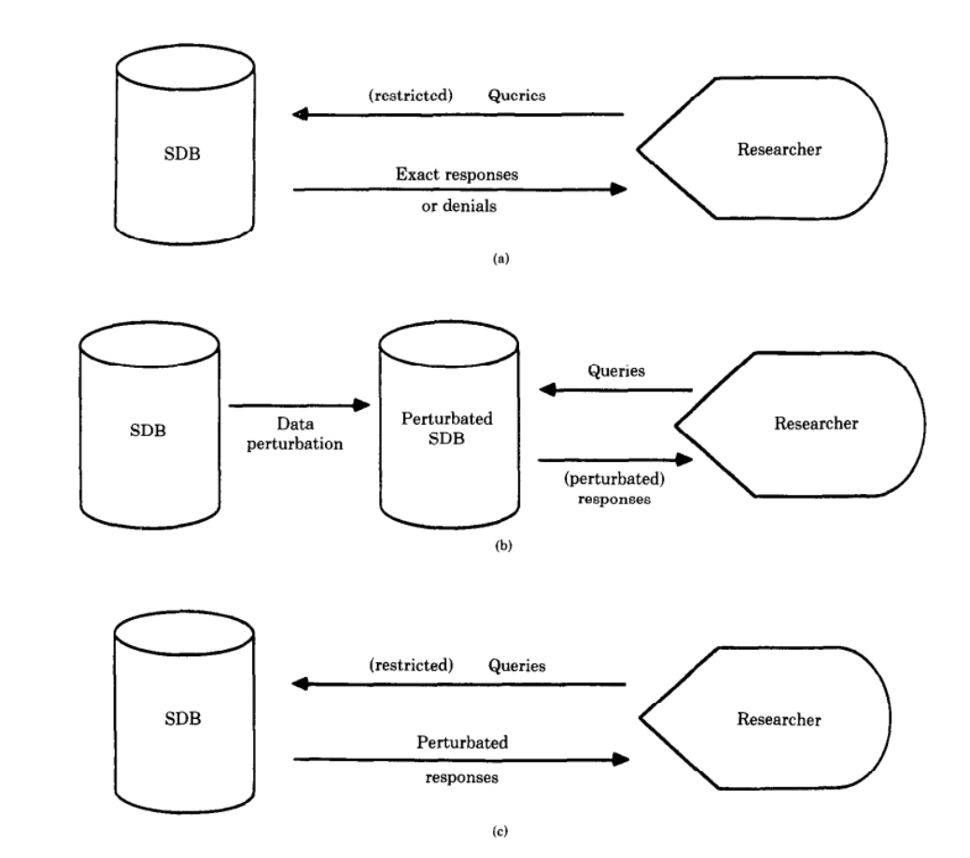
\includegraphics[width=1\linewidth]{assets/text.png}
\caption{Схемы безопасности СБД}
\label{fig:SDB_secure}
\end{figure}

\subsection{Критерии безопасности статистических баз данных}

Критерии безопасности включают оценку вероятности раскрытия записей в СБД, оценку консистентности данных при использовании методов возмущения данных и оценку зависимости между возмущением и конкретными записями. Также учитываются затраты, связанные с выполнением запросов, и назначается конкретная цена каждому запросу. Пользователям предоставляется начальная сумма, которую они могут использовать для запросов, чтобы предотвратить выведение данных.
\\

Когда речь идет о критериях безопасности, необходимо отметить, что полной гарантии безопасности в статистических базах данных (СБД) достичь невозможно. Вместо этого проводится оценка важности деанонимизированных данных и статистической точности, учитывая предпринятые меры по защите данных.
\\

Критерий безопасности "Security" оценивает вероятность раскрытия (включая частичное раскрытие) записи в СБД. Для каждого разрешенного агрегирующего запроса проводится оценка критерия безопасности. Основываясь на количестве информации в базе данных, можно определить, сколько запросов требуется для деанонимизации данных. На основе этой оценки определяется минимальный размер выборки для таких запросов.
\\

Критерий безопасности "Consistency" оценивает консистентность данных для методов возмущения данных. Оценивается степень возмущения данных путем создания агрегирующего запроса и измерения его изменений после внесения возмущений. 
\\

Критерий безопасности "Robustness" оценивает зависимость между возмущением и конкретными записями. Желательно, чтобы возмущение не зависело от данных, однако необходимо сохранить статистические свойства данных.
\\

Критерий безопасности "Costs" определяет конкретную стоимость каждого запроса. Пользователю предоставляется начальная сумма, которую он может использовать для запросов, чтобы предотвратить вывод данных. Этот критерий скорее представляет собой метод управления, а не непосредственный критерий безопасности.
\\

Таким образом, применение критериев безопасности в СБД позволяет оценивать уровень безопасности, учитывая важность данных, статистическую точность, консистентность, робастность и стоимость запросов.
\\

Исходя из вышеизложенных глав, можем убедиться, что безопасность статистических баз данных является сложной задачей, но существуют различные подходы и методы для обеспечения безопасности данных. Каждый подход имеет свои преимущества и недостатки, и выбор методов безопасности должен основываться на анализе конкретных требований и контекста использования СБД. Оценка важности данных, статистической точности и затрат помогает принять решение о применении конкретных методов обеспечения безопасности.

